\documentclass[a4paper,12pt]{article}

\usepackage[utf8]{inputenc} % Кодировка utf8
\usepackage[english, russian]{babel} % Языки: русский, английский
\usepackage{textcase}
\usepackage{geometry}
\usepackage{graphicx}
\usepackage{epstopdf}
\epstopdfsetup{update} 
\graphicspath{{}} 
\geometry{a4paper,top=2cm,bottom=2cm,left=1cm,right=1cm}


\title{Вычисление статистик $\pi, \lambda, c$ на графе}
\date{}
\author{Миронович Светлана}
 
\begin{document}
  \maketitle

Пусть у нас есть ориентированный граф, ребрам которого приписаны веса 0 или 1. Кратчайшим, оптимальным или самым дешевым будем называть такой путь в графе, что сумма ребер, входящих в этот путь (сколько раз ребро входит в путь, столько раз его вес суммируется), наименьшая.

Пронумеруем вершины в графе и пусть эти номера будут метками каждой из вершин, а также обозначим через $weight(a,b)$ вес ребра, ведущего из a в b. 

\textbf{Задача}:

Найти такой цикл в графе, что вес цикла, деленный на его длину, будет наименьшим. Такой цикл назовем оптимальным.

Заметим следующее: любой достаточно длинный по количеству ребер кратчайший путь будет представлять собой несколько ребер до вхождения в цикл, хождение по циклу и затем несколько ребер от цикла до конечной вершины, в которой заканчивается путь. В качестве примера рассмотрим следующий граф:

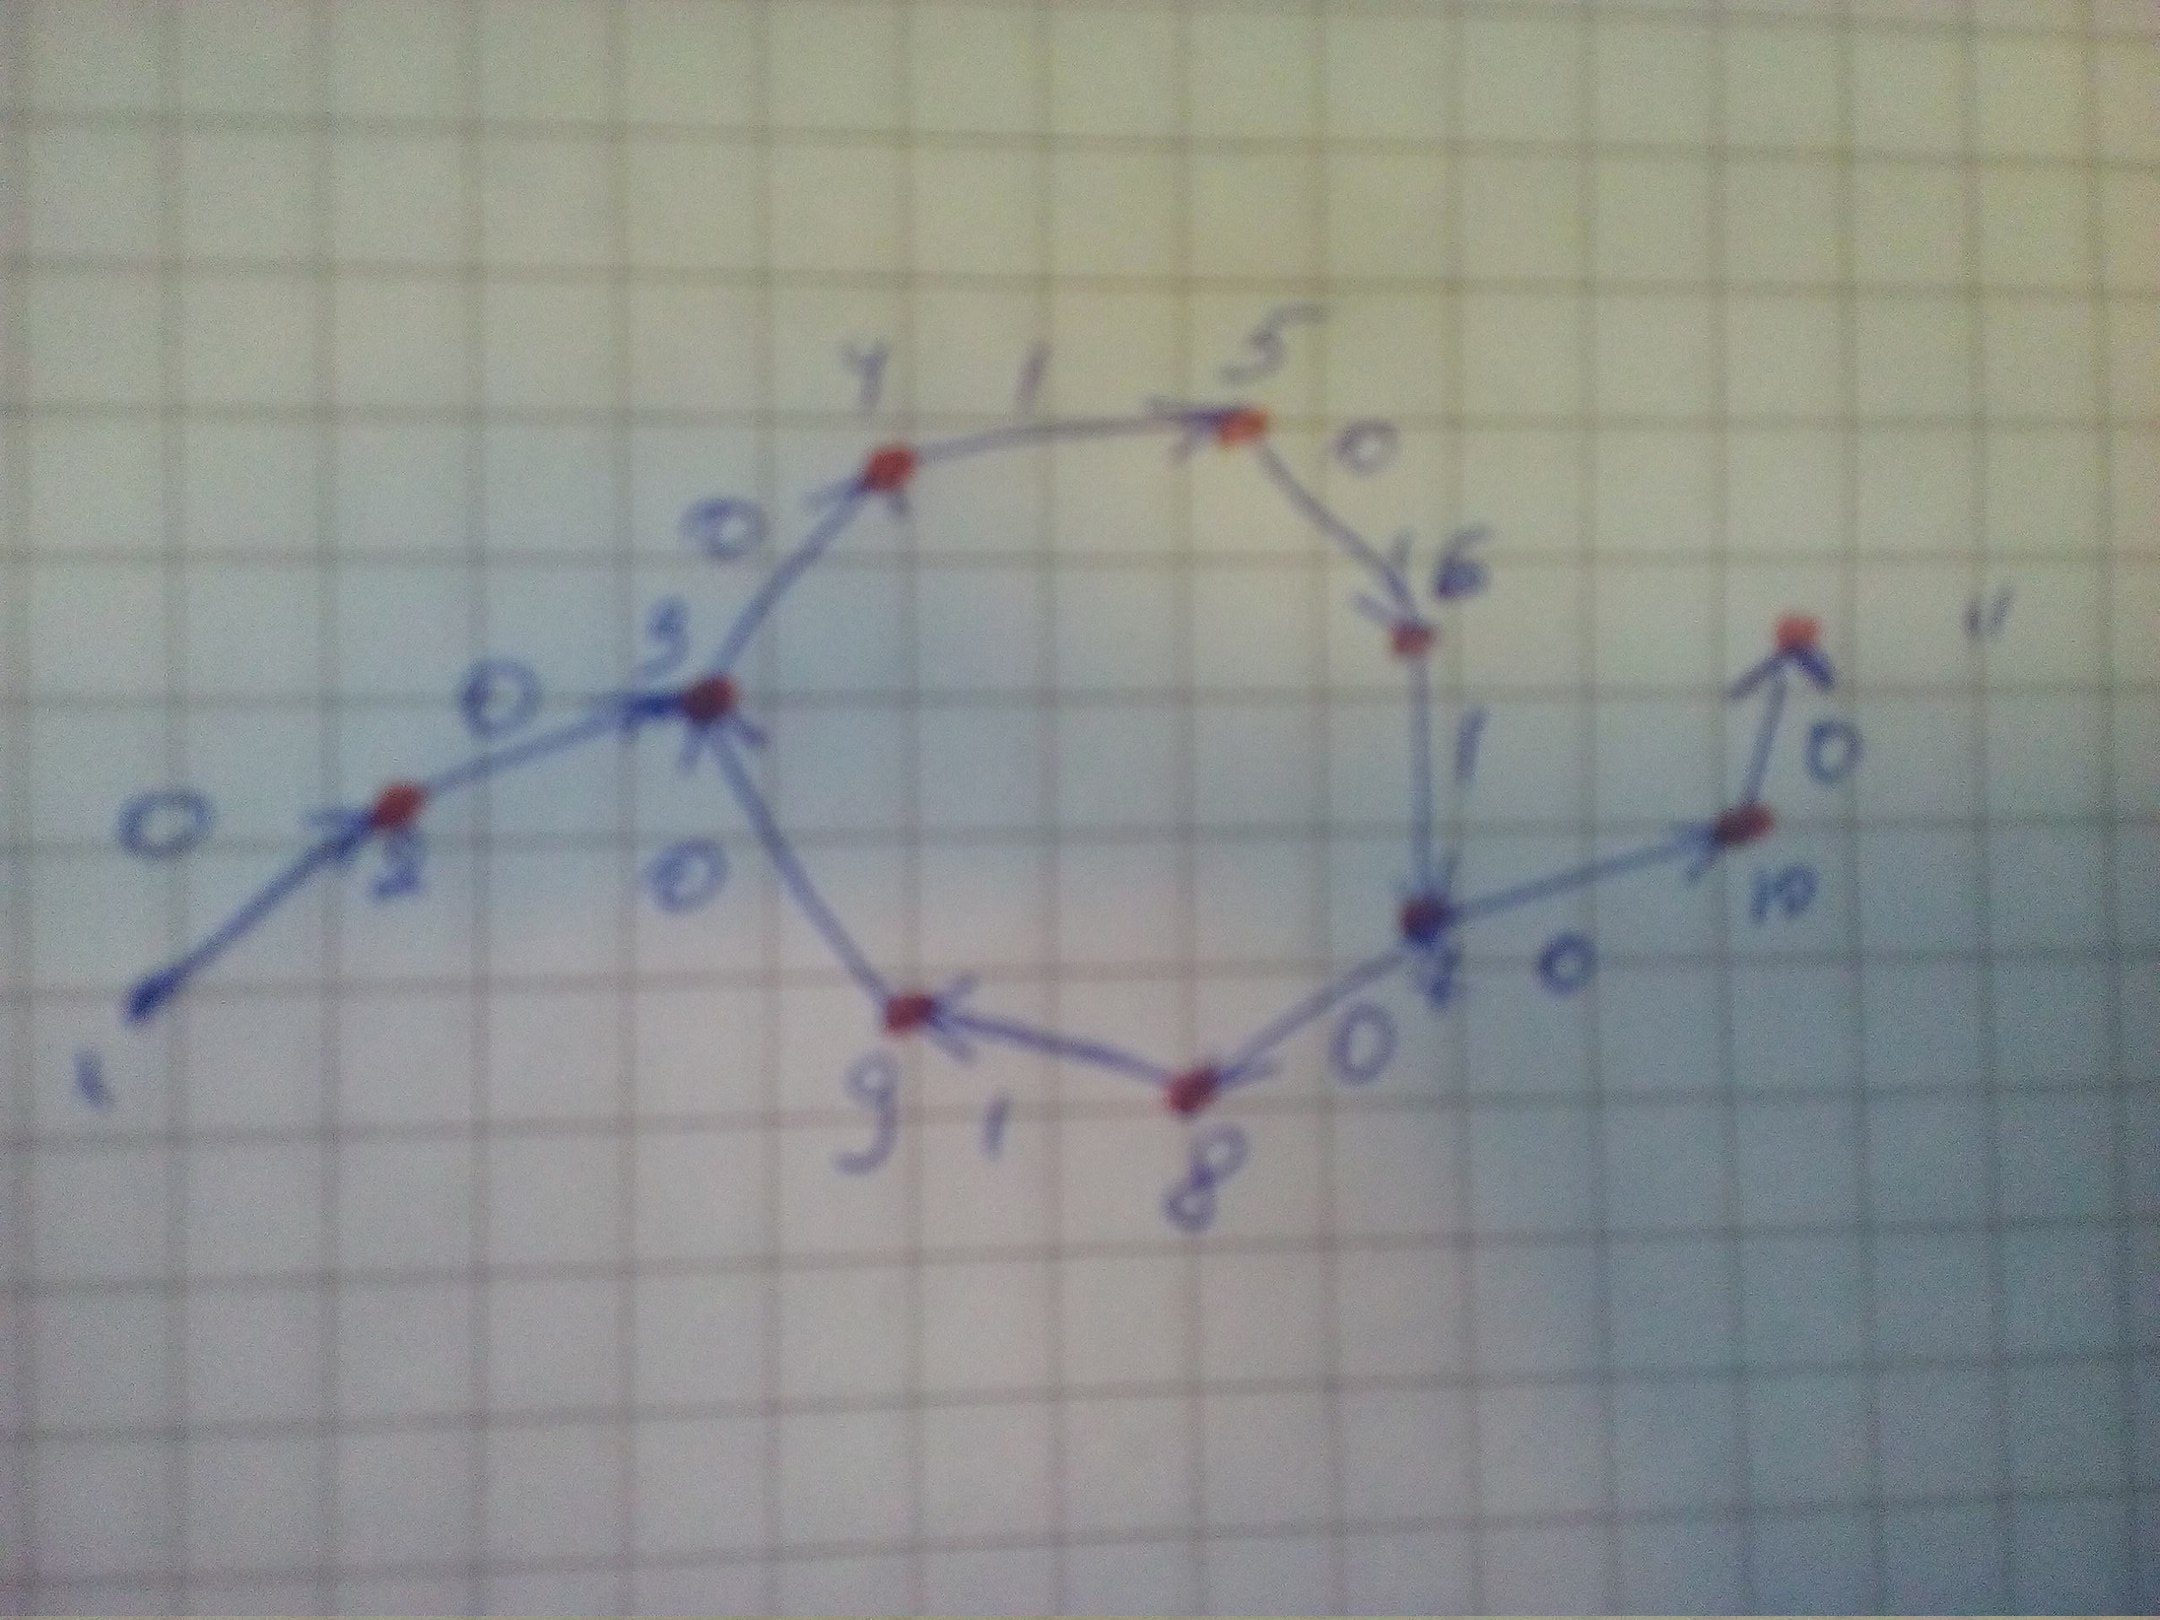
\includegraphics[width=\textwidth]{1}

По этому графу видно, что вес кратчайшего пути длины 22 будет равен 8. Здесь предцикл - это два ребра, из 1 в 2 и из 2 в 3. Цикл здесь - это перемещения по вершинам 3, 4, 5, 6, 7, 8, 9. Путь заканчивается в вершине 11, и чтобы добраться до нее. мы должны пройти по ребрам из 7 в 10 и из 10 в 11, которые не являются частью цикла.

 Соответственно цикл всегда является частью любого кратчайшего пути, начиная с некоторой длины пути $l$, считая по ребрам. Заметим, что длина цикла по ребрам не может быть больше n, а также длина предцикла и последовательность ребер после цикла также не могут быть в сумме больше, чем n. Следовательно, при длине $l \ge 2n$ мы гарантированно внутри пути хотя бы один раз полностью пройдем цикл.

Давайте разобьем задачу на 2 этапа:

\begin{itemize}
\item Нахождение самого дешевого пути в графе из k ребер до каждой из вершин
\item По найденному пути вычленение цикла, по которому этот путь ходит
\end{itemize}

\textbf{Нахождение самого дешевого пути из k ребер}

Для каждой из вершин мы бы хотели знать кратчайший путь из k ребер, который заканчивается в этой вершине, но нам не важно, где начинается этот путь. Важно только, чтобы путь не содержал петель.

Построим наш алгоритм нахождения кратчайших путей на следующем инварианте: на каждом этапе алгоритма k мы будем знать кратчайшие пути из k ребер до каждой из вершин. Пусть $d_k[i]$ на шаге k хранит вес кратчайшего пути из k ребер, ведущего в вершину i, а $p_k[i]$ хранит вершину, из которой было проведено последнее ребро из данного кратчайшего пути. Например, пусть у нас есть кратчайший путь $1 \rightarrow 2 \rightarrow 3 \rightarrow 4$ с весами ребер соответственно 0, 1, 1. Тогда $d_3[4] = 2, p_3[4] = 3$. 

На нолевом шаге алгоритма заполняем $d_0$ нулями, $p_0$ минус единицами. Мы так поступаем, поскольку кратчайший путь из 0 ребер - это просто оставаться в той же вершине без движения. Соответственно вес такого пути 0 (и такой путь можно построить для каждой вершины), и при этом такой путь ниоткуда не идет, соответственно мы не можем указать в $p_0$ настоящие вершины.

Переход от этапа k к этапу k+1 будет выглядеть следующим образом: заполним сначала $d_{k+1}$:
 $$d_{k+1}[i] = +\infty, p_{k+1}[i] = -1  \forall i = \overline{1,n}$$

Далее пройдемся по всем ребрам. Для каждого ребра мы знаем вершину a, откуда идет это ребро, вершину b, куда ведет это ребро, и вес c данного ребра. В таком случае для каждого ребра мы будем совершать следующее действие:
$$if~ d_{k+1}[b] > d_{k}[a] + c~ then~ d_{k+1}[b] = d_{k}[a] + c, p_{k+1}[b] = a$$

Соответственно в $d_{k+1}$ всегда хранится вес какого-то пути длины k+1, и с прохождением по всем ребрам этот вес только улучшается (и вес, равный бесконечности, означает, что пути из k+1 ребра нет). Докажем по индукции, что в конце этапа $k+1$ у нас всегда в $d_{k+1}$ хранятся наилучшие веса.

База индукции: на нулевом шаге хранятся наилучшие веса. Действительно, поскольку веса ребер у нас неотрицательные, то и вес всего пути не может быть отрицательным. Следовательно, вес пути равный нулю является наилучшим достижимым, и именно нули хранятся в $d_0$.

Индуктивны шаг: пусть на шагах 0, 1, 2, ..., k мы нашли отпимальные пути. Докажем, что и на $k+1$ шаге у нас будут найдены оптимальные пути. Пусть у нас есть некоторое количество путей из k+1 ребра, ведущие в вершину v. Положим от противного, мы выбрали неоптимальный путь, т.е. $\exists v_x, d_k[v_x] + weight(v_x, v) < d_{k+1}[v]$ (а как мы помним, по предположению индукции, в $d_k[v_x]$ уже хранится вес оптимального пути из k ребер, ведущий в $v_x$). Но поскольку когда мы проходили по всем ребрам, мы также и прошли по ребру $(v_x, v)$, то мы обязательно должны были взять это ребро, и тогда бы обязательно в $d_{k+1}[v]$ хранилось бы $d_{k+1}[v] = d_{k}[v_x] + weight(v_x, v)$. Противоречие.

\textbf{Нахождение цикла по пути}

Поскольку в графе может быть несколько циклов, по которым бы ходили оптимальные пути (такое возможно, например, когда граф несвязный), нам следует найти все такие циклы и из них выбрать оптимальный. В таком случае, будем поступать следующим образом: для каждой вершины будем восстанавливать ее оптимальный путь до тех пор, пока не встретим вершину, в которой уже побывали. Когда мы повстречаем такую вершину, это будет означать, что мы замкнули цикл. По векторам $d_k$ мы всегда сможем вычислить вес цикла, и соответственно, мы будем сравнивать каждый найденный цикл с найденными ранее. Если найденный цикл "оптимальнее", то оставим только его, остальное выкинем. Если же он не является более оптимальным по отношению веса к длине, то мы забываем этот цикл. Подобную операцию нахождения циклов проделываем для каждой из вершин.

Заметим, что непременно найдется вершина, в которую ведет путь, содержащий оптимальный цикл. Это следует из того, что в пределе оптимальным путем является путь, который ходит по циклу. Поскольку мы доказали, что на каждом этапе алгоритма мы находим оптимальные пути из k ребер (и более того, все последующие пути из k+1, k+2, ... ребер строятся на оптимальных путях из $k$ ребер), то оптимальные пути из $k$ ребер, начиная с $k \ge 2n$, обязательно проходят оптимальный цикл.

Алгоритмически нахождение цикла по путям выглядит следующим образом:

\begin{itemize}
\item Восстанавливать путь из вершины до того момента, пока мы не встретили уже ранее виденную вершину
\item Вычислить отношение веса к длине цикла на основании векторов $d_k$
\item Сравнить это отношение с отношениями ранее найденных циклов и оставить только наилучшее
\end{itemize}  

textbf{Ассимптотическая сложность}

Нахождение всех кратчайших путей потребует $2n$ этапов нахождения $d_k$, каждый из которых требует m шагов. Следовательно, нахождение оптимальных путей достаточной для нас длины имеет сложность $O(nm)$.

Восстановление одного пути с целью нахождения цикла требует не более $O(n)$, и таких восстановление требуется $n$, следовательно, общая сложность нахождения оптимального цикла по построенным путям имеет сложность $O(n^2)$.

Итого, общая сложность алгоритма будет $O(mn + n^2) = O(n(m+n))$.

В нашем случае обычно $m ge n$, и в таком случае сложность упрощается до $O(mn)$.
\end{document}